\documentclass[../../main]{subfiles}

\begin{document}
\section{SIMULATION ENVIRONMENT}
\lstset{language=XML}
\section{Introduction to the Simulation Environment}
In developing a control strategy for mobile robots such as Automated Guided Vehicles (AGVs),
simulation plays a crucial role in testing software components, robot behavior, and control algorithms across various environments. 
Before physically building the robotic system, running a simulation provides a risk-free and cost-effective approach to refining 
its design and functionality. By simulating the robot's behavior in a controlled virtual environment, different algorithms can 
be tested and optimized to ensure efficient navigation, obstacle avoidance, and perception without the risk of hardware damage. 

The simulation environment was built using the \textbf{Robot Operating System (ROS)} 
and the \textbf{Gazebo} simulator, with the \texttt{gazebo\_ros} 
package. \texttt{RViz} was utilized for real-time visualization of sensor data and robot trajectories, 
while \texttt{OpenCV} handled computer vision tasks such as \textit{line following} and \textit{QR code detection}. The following sections provide 
detailed insights into their implementation and role in the project.\\
% the next paragraph needs to be revised 
\newpage
\section{Tools and Framework}
\subsection{Gazebo}

Gazebo was initially developed in 2002 to facilitate the simulation of ground robot applications in both indoor and outdoor environments \cite{koenig2004design}. 
Over the years, it has evolved into a mature open-source project widely adopted by the global robotics community for various applications. 
Gazebo follows a modular architecture, incorporating four key components essential for robot simulation:

\begin{itemize}
    \item \textbf{Physics Engine Support} – Gazebo integrates multiple physics engines to handle collision detection, contact dynamics, and reaction forces between rigid bodies.
    \item \textbf{Sensor Simulation} – It provides a comprehensive library of commonly used robotic sensors, including cameras, LiDAR, sonar, GPS, and IMUs, 
    along with configurable noise models for realistic sensor emulation.
    \item \textbf{Multiple Interfaces} – The simulator supports various interfaces for programmatic interaction, including C++ for developing plugins.
    \item \textbf{Graphical User Interface (GUI)} – Gazebo features an interactive 3D environment that enables users to visualize and manipulate the simulated world in real-time.
\end{itemize}

\begin{figure}[H]
    \centering

\includegraphics[width=0.7\textwidth]{fig/gazebo_logo.png}
\caption{Gazebo Simulator}
\label{Gazebo logo} % Unique label for referencing
\end{figure}
\newpage
Gazebo is a robust simulation tool integrated with the Robot Operating System (ROS),
designed to simulate robotic and sensor applications in both indoor and outdoor 3D environments. 
It follows a Client-Server architecture coupled with a topic-based Publish/Subscribe model for inter-process communication, 
enabling efficient data exchange between the various components of the system.

For dynamic simulations, Gazebo leverages several high-performance physics engines, 
including the Open Dynamics Engine (ODE)\cite{smith2016}, Bullet\cite{bullet2016}, Simbody\cite{simbody2016}, and the Dynamic Animation and Robotics Toolkit (DART)\cite{dart2016}. 
These engines handle rigid-body physics simulations, providing highly accurate interactions between objects. 
Additionally, Gazebo employs the Object-Oriented Graphics Rendering Engine (OGRE)\cite{ogre2016} for 3D graphics rendering, 
generating realistic visual environments that enhance the simulation experience.

In this architecture, the Gazebo Client sends control data, such as the coordinates of simulated objects, 
to the Server, which then manages real-time control of the virtual robot. Gazebo also supports distributed simulation, 
allowing the Client and Server to run on separate machines, which can be beneficial for scaling and performance.

\begin{figure}[H]
    \centering
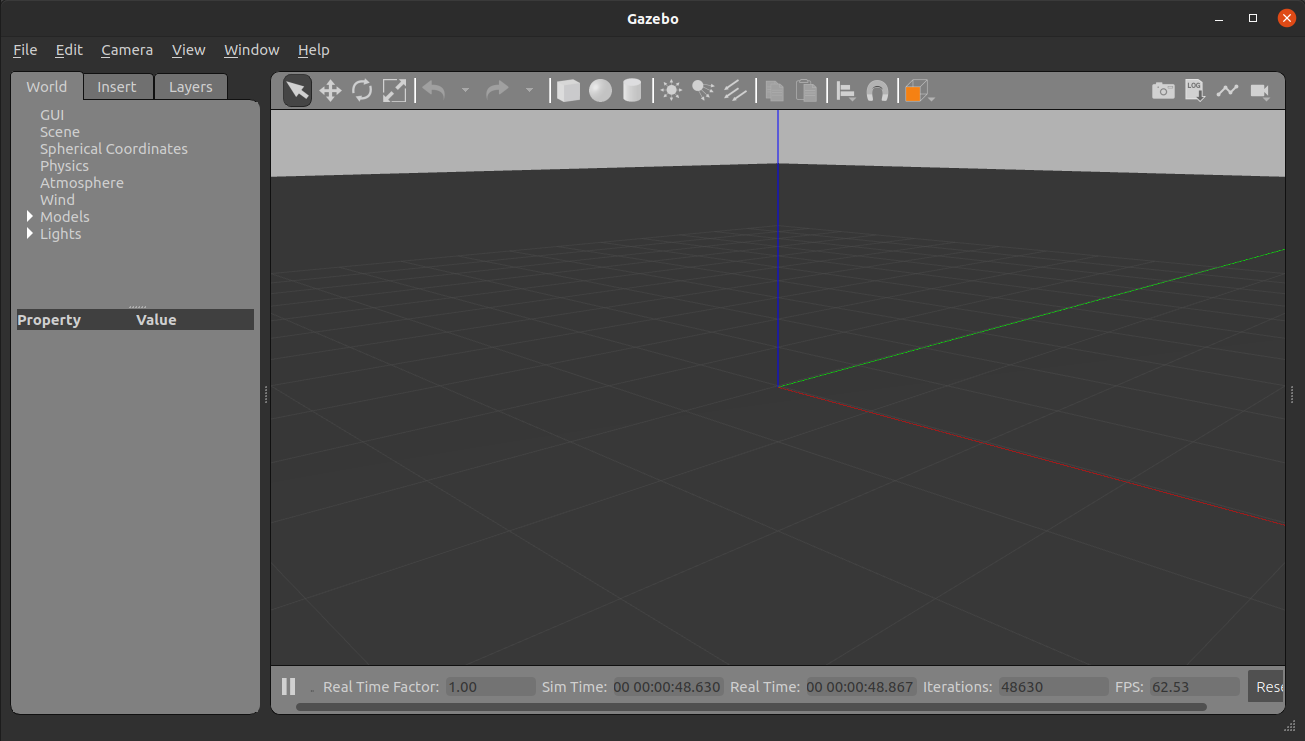
\includegraphics[width=\textwidth]{fig/gazebo_empty_world.png}
\caption{Empty world in Gazebo}
\label{Gazebo empty world} % Unique label for referencing
\end{figure}

The ROS Plugin for Gazebo ensures  integration between the two platforms, enabling direct communication with ROS. 
This allows both simulated and real robots to be controlled using the same software interface, making Gazebo an ideal platform for testing, 
developing, and validating robotic systems in a virtual environment before deployment on physical hardware.

This plugin facilitates bi-directional communication through ROS topics, services, and actions, allowing sensor data from Gazebo—such as LiDAR, 
cameras, and IMUs—to be published as ROS messages while also enabling ROS-based velocity and trajectory commands to control simulated robots. 
Additionally, the plugin supports \texttt{ros\_control}, making it possible to implement position, velocity, and effort controllers, 
which are essential for tuning PID loops before testing them on real actuators.

\begin{minted}{xml}
    <launch>
  <arg name="model" default="$(env TURTLEBOT3_MODEL)" doc="model type [burger, waffle, waffle_pi]"/>
  <arg name="x_pos" default="0.0"/>
  <arg name="y_pos" default="0.0"/>
  <arg name="z_pos" default="0.0"/>

  <include file="$(find gazebo_ros)/launch/empty_world.launch">
    <arg name="world_name" value="$(find turtlebot3_gazebo)/worlds/empty.world"/>
    <arg name="paused" value="false"/>
    <arg name="use_sim_time" value="true"/>
    <arg name="gui" value="true"/>
    <arg name="headless" value="false"/>
    <arg name="debug" value="false"/>
  </include>

  <param name="robot_description" command=
  "$(find xacro)/xacro --inorder 
$(find turtlebot3_description)/
urdf/turtlebot3_$(arg model).urdf.xacro" />

  <node pkg="gazebo_ros" type="spawn_model" name="spawn_urdf" args="-urdf -model turtlebot3_$(arg model) -x $(arg x_pos) -y 
  $(arg y_pos) -z $(arg z_pos) -param robot_description" />
</launch>
\end{minted}
The provided example demonstrates how the \textbf{ROS Plugin for Gazebo} enables the spawning and control of a robot model 
within a simulated environment, enabling \textbf{smooth and efficient integration} with the \textbf{Robot Operating System (ROS)}. 
The launch file initializes an empty \textbf{Gazebo} world and loads a robot model described in a 
\textbf{URDF (Unified Robot Description Format)} file using the \texttt{spawn\_model} node from the \texttt{gazebo\_ros} package. 
Additionally, the \texttt{robot\_state\_publisher} node is included to publish the robot’s joint states, 
ensuring that its transformations can be visualized and utilized in \textbf{ROS-based frameworks} such as \textbf{MoveIt} or \textbf{RViz}. 
This integration allows developers to test \textbf{robot behaviors, sensor data integration, and control algorithms} in a virtual environment 
before deploying them on physical hardware.  

It facilitates bi-directional communication through \textbf{ROS topics, services, and actions}, 
enabling sensor data from Gazebo—such as \textbf{LiDAR, cameras, and IMUs}—to be published as \textbf{ROS messages} 
while also allowing \textbf{ROS-based velocity and trajectory commands} to control simulated robots. 
Additionally, the plugin supports \textbf{ros\_control}, enabling the implementation of \textbf{position, velocity, and effort controllers}, 
which are essential for tuning \textbf{PID loops} before applying them to real actuators.  

This specific example shows a \textbf{ROS launch file} that spawns a \textbf{TurtleBot3} model shown\\ ~\cref{TurtleBot3 in empty world} in an empty \textbf{Gazebo} simulation environment. 
This file provides flexibility by allowing users to specify the \textbf{TurtleBot3 model type} (\texttt{burger}, \texttt{waffle}, or \texttt{waffle\_pi}) 
and configure the \textbf{robot's initial position}. It also sets critical simulation parameters, 
such as \textbf{enabling GUI rendering, synchronizing ROS time with Gazebo simulation time, 
and dynamically loading the robot’s description} based on the selected model type. 
The launch file ensures a well-structured simulation environment where \textbf{robotic software, motion planning, and perception algorithms} 
can be tested under realistic conditions. 

\begin{figure}[H]
    \centering
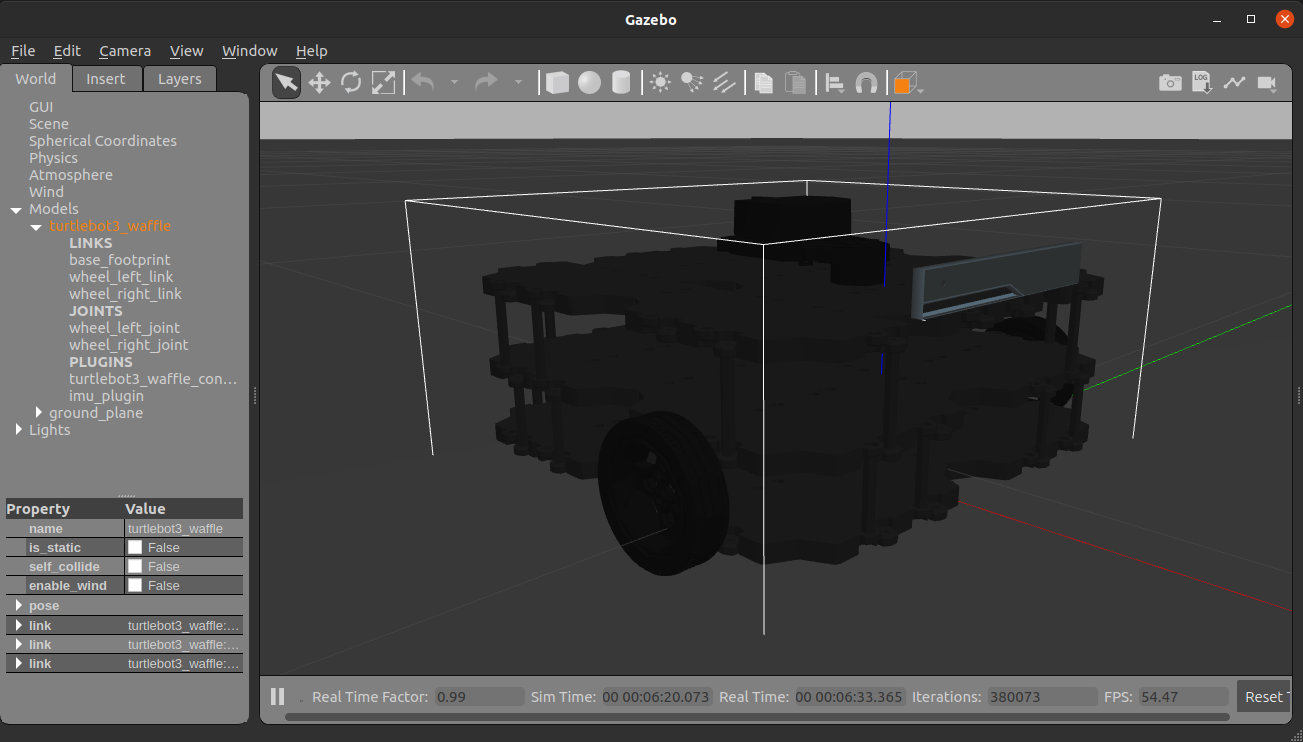
\includegraphics[width=\textwidth]{fig/turtlebot3_waffle.png}
\caption{TurtleBot3 Waffle spawned in empty world}
\label{TurtleBot3 in empty world} % Unique label for referencing
\end{figure}

The Gazebo Graphical User Interface (GUI) provides an interactive environment for users to visualize and manipulate their simulated worlds in real-time. 
One of the key features of the GUI is the set of side tabs, which organize various tools and functionalities. Among these, the left side pannel that appears \cref{Left side pannel} World, Insert, 
and Layers tabs are particularly important for managing the simulation environment and objects within it.

The \textbf{World Tab} in Gazebo’s GUI allows users to manage and configure the 
properties of the simulation world, providing several options for modifying the 
environment settings. Users can adjust the \textbf{gravity settings} to control the 
strength of gravity in the simulation, select the \textbf{physics engine} (such as 
\textbf{ODE}, \textbf{Bullet}, or \textbf{DART}) to determine the level of simulation 
fidelity and performance, and customize \textbf{time and weather conditions}, including 
factors like sunlight, fog, and rain. Additionally, the World tab provides detailed 
information about the models within the simulation, including their \textbf{joints} and 
\textbf{links}. Users can visualize and modify the connections between different parts 
of a robot or object, defining how they move and interact with each other. The 
\textbf{links} represent rigid bodies, while \textbf{joints} define the relative motion 
between those bodies, such as revolute, prismatic, or fixed joints. This tab plays a 
crucial role in fine-tuning the simulation environment and robot behavior, ensuring that 
the simulation behaves as expected for the application at hand. It is an essential tool 
for accurately replicating real-world conditions and testing robotic systems in varied 
scenarios.

The \textbf{Insert Tab} allows users to add various objects and 
components to the simulation environment. Users can insert robot models, lights, 
sensors, and even other world elements, which helps populate the simulation for 
testing and development. Additionally, the tab makes it easy to add custom plugins 
or adjust the robot's attributes in the virtual world.

The \textbf{Layers Tab} provides control over the visibility of 
different elements within the simulation. Users can toggle the visibility of models, 
sensors, and other objects in the scene to focus on specific parts of the simulation. 
This helps streamline the workspace, especially when dealing with complex environments 
and large-scale simulations.

\begin{figure}[H]
    \centering
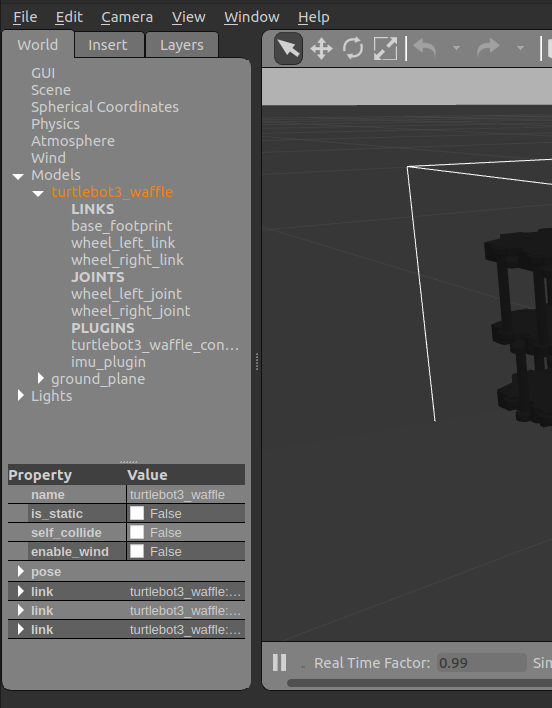
\includegraphics[width=0.55\textwidth]{fig/gui_left_tab.png}
\caption{Gazebo Graphical User Interface left side pannel}
\label{Left side pannel} % Unique label for referencing
\end{figure}

The lower part of the Gazebo GUI displayed in \cref{Lower part} provides critical real-time simulation information 
and performance metrics. One of the most important features is the \textbf{Real-Time 
Factor (RTF)}, which indicates the ratio between real-time and simulated time. This 
factor helps users determine how efficiently the simulation is running, with values 
close to 1.0 indicating that the simulation is running in real-time. If the RTF is 
greater than 1.0, it suggests that the simulation is running faster than real time, 
while a value less than 1.0 indicates that it is running slower.

In addition to RTF, it also displays \textbf{Sim Time}, which 
shows the simulation's elapsed time. This is useful for tracking the progression of 
events in the simulation and synchronizing it with other systems. The \textbf{Real Iterations} 
and \textbf{Sim Iterations} counters provide insight into the number of iterations performed 
by the simulation per second for real-time and simulated time, respectively. Monitoring 
these values helps users assess the efficiency of the simulation and diagnose performance 
issues if the simulation is not proceeding as expected.

\begin{figure}[H]
    \centering
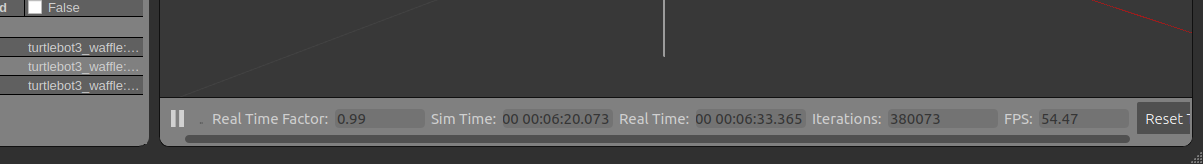
\includegraphics[width=\textwidth]{fig/gui_lower_part.png}
\caption{Gazebo Graphical User Interface lower part}
\label{Lower part} % Unique label for referencing
\end{figure}

The top part of the Gazebo GUI (\cref{Top part}) provides several essential controls and information 
related to the simulation’s overall operation. At the top-left corner, users will find the 
\textbf{File} menu, which includes options to open, save, and manage Gazebo worlds. 
It also allows users to load and save configurations, and set preferences for simulation 
settings. 

In addition, the top part of the GUI provides options for manipulating the lighting 
within the simulation. Users can select from \textbf{Point}, \textbf{Spot}, and 
\textbf{Directional} lights to illuminate different parts of the world. Point lights 
emit light in all directions from a single point, Spot lights create a focused beam 
of light, and Directional lights simulate sunlight, casting parallel rays in a 
specific direction. This allows for realistic and customizable lighting in the 
simulation environment. 

The \textbf{Selection Light} tool enables users to adjust the lighting between 
two or more objects in the simulation, offering more control over how objects are 
illuminated and how shadows are cast in the environment. 

Moreover, the GUI allows users to switch between different \textbf{perspective views}, 
such as top-down, side, or camera views, to inspect and interact with the simulation 
from different angles. 

\begin{figure}[H]
    \centering
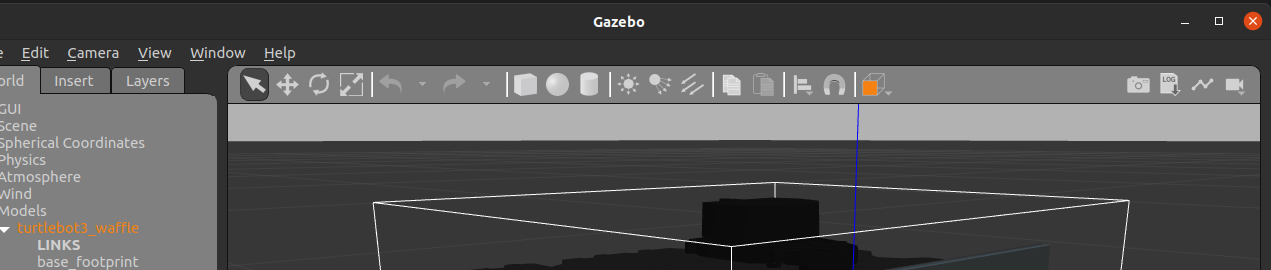
\includegraphics[width=0.8\textwidth]{fig/gui_top_part.png}
\caption{Gazebo Graphical User Interface top part}
\label{Top part} % Unique label for referencing
\end{figure}

Right-clicking on an object in the Gazebo simulation environment brings up a context-sensitive 
menu that allows users to perform a variety of actions to interact with and manipulate the object. 
The options available in this menu include:

1. \textbf{Move To}: This option allows users to move a selected object to a specified location 
in the simulation world. After selecting this option, users can click on a point in the world to 
which the object will be moved, making it easier to position objects accurately within the 
environment.

2. \textbf{Follow}: The Follow option enables users to make the camera follow a particular 
object in the simulation. When this option is activated, the camera will automatically track 
the movement of the selected object, allowing users to observe its behavior from a fixed 
perspective, which can be useful when testing robot movements or simulating dynamic 
scenarios.

3. \textbf{Edit}: The Edit option opens a set of interactive tools that allow users to modify 
the properties of the selected object, such as its position, orientation, size, and material 
properties.

\begin{figure}[H]
    \centering
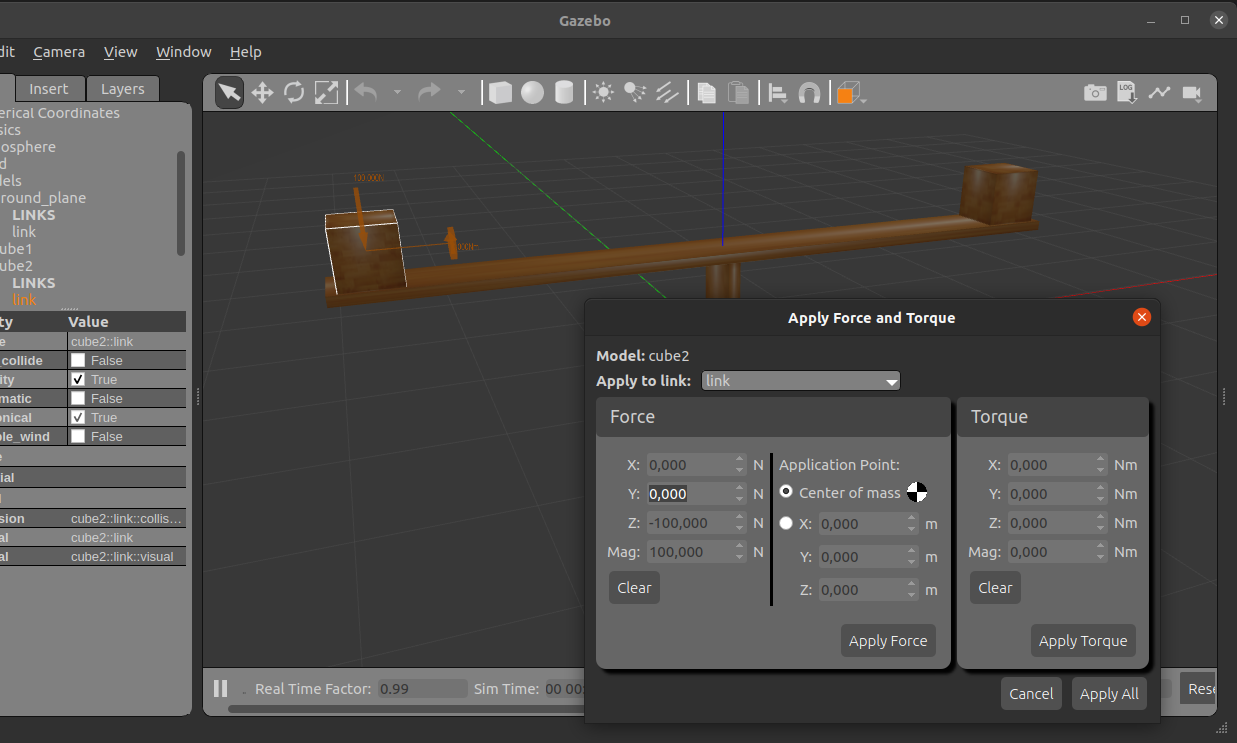
\includegraphics[width=0.6\textwidth]{fig/seesaw_example.png}
\caption{Example of force applied on one side of a seesaw in gazebo}
\label{Seesaw} % Unique label for referencing
\end{figure}

4. \textbf{Apply Force/Torque}: This option gives users the ability to apply a force or 
torque to the selected object, which is especially useful for testing how the object reacts 
under various physical conditions.\cref{Seesaw} shows how users can specify the direction, magnitude, and duration 
of the applied force or torque, allowing for controlled experiments on the object’s behavior 
within the simulated environment.
\newpage
\subsection{RViz}
\textbf{RViz} (ROS Visualization) is an open-source 3D visualization tool that provides real-time graphical representations of robotic systems. 

\begin{figure}[H]
    \centering
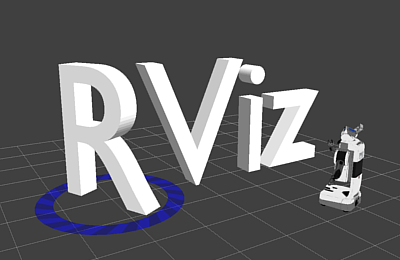
\includegraphics[width=0.65\textwidth]{fig/rviz_logo.png}
\caption{Rviz (Ros Visualization)}
\label{Rviz Logo} % Unique label for referencing
\end{figure}

It serves two primary purposes: (1) visualizing sensor data, such as LiDAR scans, point clouds from 3D sensors (e.g., RealSense, Kinect), 
and camera images, in an intuitive 3D environment; and (2) enabling interactive control of robotic systems by sending commands 
like navigation goals or waypoints. In this project, RViz was used extensively to monitor sensor outputs, validate navigation algorithms, 
and debug the robot’s behavior during simulation. Its seamless integration with ROS topics and plugins made it an indispensable tool for 
visualizing complex data streams, such as laser range finder (LRF) distances and Point Cloud Data (PCD), without requiring additional programming.  
\newpage
\section{Implementation of the Simulation Environment}

The implementation of the simulation environment is carefully designed to ensure that the 
results obtained in simulation closely reflect real-world performance. Most simulation 
parameters, including the robot’s dimensions, mass properties, sensor specifications, 
and environmental conditions, are selected to match the specifications outlined in the 
competition framework. This ensures that the robot developed based on simulation 
results can seamlessly transition from a virtual setting to real-world deployment with 
minimal modifications.  

A key aspect of this simulation is the accurate modeling of robot dynamics, actuator 
characteristics, and sensor behavior. The physics engine parameters, such as friction 
coefficients, and sensor noise models, are tuned to replicate real-world 
conditions as precisely as possible. Additionally, the design of the virtual environment, 
including terrain features, obstacles, and lighting conditions, is configured to match 
the competition setup. This allows for realistic testing and validation of navigation 
and control algorithms.  

By incorporating these considerations, the simulation provides a reliable testing ground 
for developing and refining motion planning, perception, and control strategies. This 
approach reduces the gap between simulated and real-world performance, ensuring that 
insights gained from the virtual environment translate effectively to the physical robot. 
However, like any simulation-based approach, there are inherent advantages and 
disadvantages when using simulators to test robot behaviors, as discussed in \cite{lera2014mobile}. 

Despite these limitations, careful selection of simulation parameters---such as physics 
engine settings, sensor noise models, and environmental conditions---enhances the accuracy 
of the virtual testing environment. The following subsections detail the implementation 
of the robot model, world design, and control and sensor integration, outlining how each 
component contributes to achieving a high-fidelity simulation.

\subsection{Robot Model ( URDF/SDF )}
\subsection{World Design} 

\begin{figure}[H]
  \centering
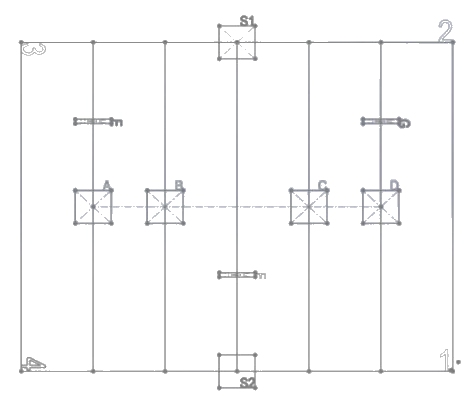
\includegraphics[width=0.7\textwidth]{fig/competition_area_layout_teknofest.png}
\caption{Teknofest competition real map layout}
\label{Teknofest competition real map layout} % Unique label for referencing
\end{figure}


The simulation environment was designed to replicate the competition layout in \cref{Teknofest competition real map layout} as closely as possible. 
The terrain was constructed using custom models to accurately mimic the competition area, incorporating key features such as a 
\textbf{white wooden floor}, \textbf{black lines for path following}, \textbf{platforms for load dynamics}, 
\textbf{obstacles}, and \textbf{friction variations} to simulate real-world conditions. 

In Gazebo, this entire environment is saved as a world file, which includes all the models, textures, 
and configurations necessary to recreate the simulation. The world file is written in the Simulation Description Format (SDF), 
an XML-based format used to describe the properties and behavior of objects and environments in Gazebo. 

SDF allows for easy definition of physical properties, geometries, lighting, and sensor configurations, making it a versatile 
and standard way to represent simulation environments. The SDF format ensures that the simulation setup is reproducible, 
shareable, and can be modified easily for different testing scenarios. Similar to the Unified Robot Description Format (URDF), 
which is used for defining robot models in ROS, SDF provides a structured way to describe objects and environments. 
While URDF focuses primarily on robot kinematics and geometry, SDF is more comprehensive and extends its capabilities 
to encompass the full environment, including physics properties, sensor configurations, and world dynamics.

The world file was made through the design of 
individual SDF files for each model within the environment. These individual 
models were first defined with each having its own dedicated 
SDF file. Once the models were completed, they were then integrated into a 
single world file, named \texttt{competition\_area.world} (in SDF format). 
This world file serves as the central configuration, bringing together all 
the models, their properties, and the environment settings.
\subsubsection{Environment Layout}  

Designed to replicate the competition area closely the world contains custom models were created to represent key elements of the space,
ensuring that the robot's interaction with its surroundings is as realistic as possible. Key components of the environment layout include the following:

\begin{itemize}
    \item \textbf{Flooring and Pathways:} A \textbf{white wooden floor} was chosen to resemble the actual competition floor, 
    providing a surface with consistent friction properties for the robot to interact with. The \textbf{black lines for path 
    following} were added on the white floor according to the competition specifications, acting as markers for the robot's autonomous 
    navigation algorithms to follow.

    \begin{figure}[H]
        \centering
    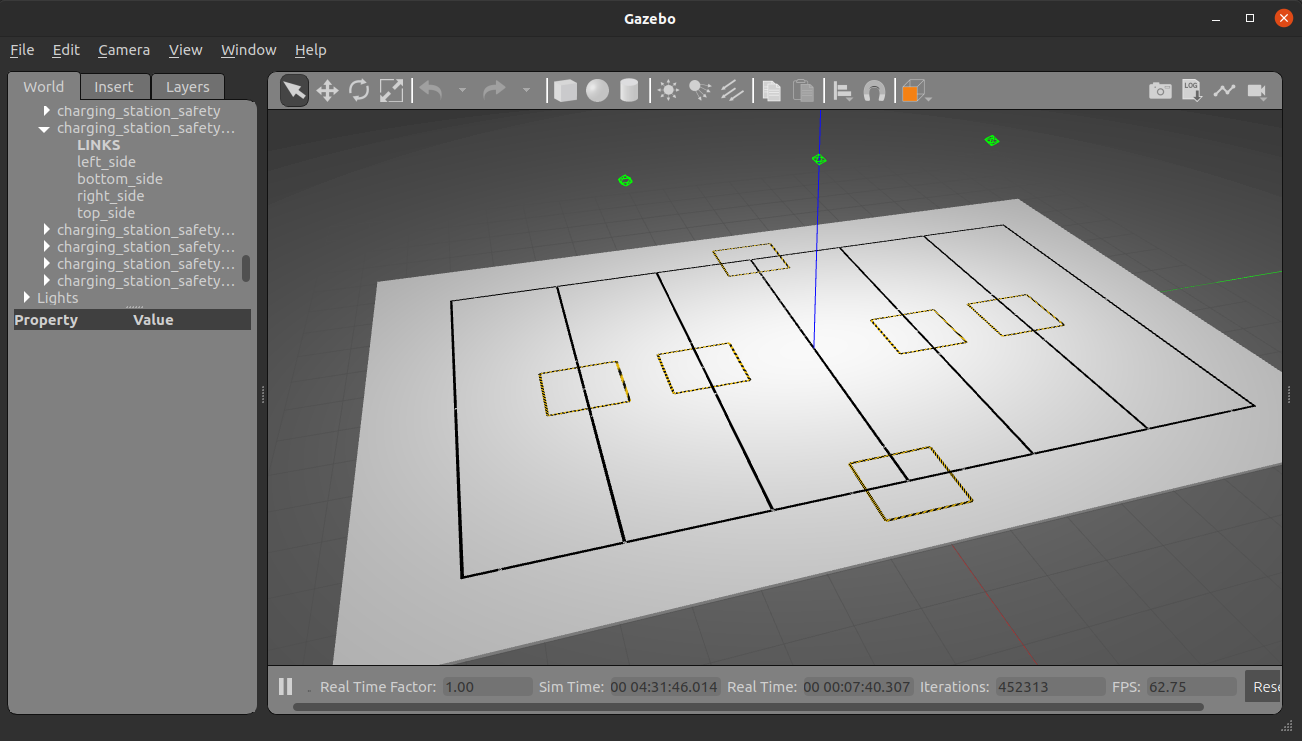
\includegraphics[width=\textwidth]{fig/white_floor.png}
    \caption{White wooden floor with black lines in gazebo}
    \label{White wooden floor} % Unique label for referencing
    \end{figure}

    The black lines for path following were also incorporated into the simulation as 
    individual objects within the Gazebo environment. Each line was treated as a separate 
    model to allow easy modifications, such as adjusting their position, length, or 
    orientation, without affecting the rest of the simulation environment. This modular 
    approach makes it easier to tweak the lines for different test scenarios, ensuring 
    flexibility and quick adjustments during development and testing.
    
    \begin{minted}{xml}
        ...
        <wall_time>1738074256 296636706</wall_time>
        <iterations>117145</iterations>
        <model name='black_line'>
          <pose>0 0 0.06 0 -0 0</pose>
          <scale>1 1 1</scale>
          <link name='line_link'>
            <pose>0 0 0.06 0 -0 0</pose>
            <velocity>0 0 0 0 -0 0</velocity>
            <acceleration>0 0 0 0 -0 0</acceleration>
            <wrench>0 0 0 0 -0 0</wrench>
          </link>
        </model>
        <model name='black_line_clone'>
          <pose>0 2.33333 0.06 0 -0 0</pose>
          <scale>1 1 1</scale>
          <link name='line_link'>
            <pose>0 2.33333 0.06 0 -0 0</pose>
            <velocity>0 0 0 0 -0 0</velocity>
            <acceleration>0 0 0 0 -0 0</acceleration>
            <wrench>0 0 0 0 -0 0</wrench>
          </link>
        </model>
        <model name='black_line_clone_0'>
          <pose>0 4.666 0.06 0 -0 0</pose>
          <scale>1 1 1</scale>
          ...
    \end{minted}

    Additionally, QR code tags were placed at key locations, such as loading/unloading points, stations, and before 
    turns, to provide the robot with precise location information.

    \begin{figure}[H]
        \centering
    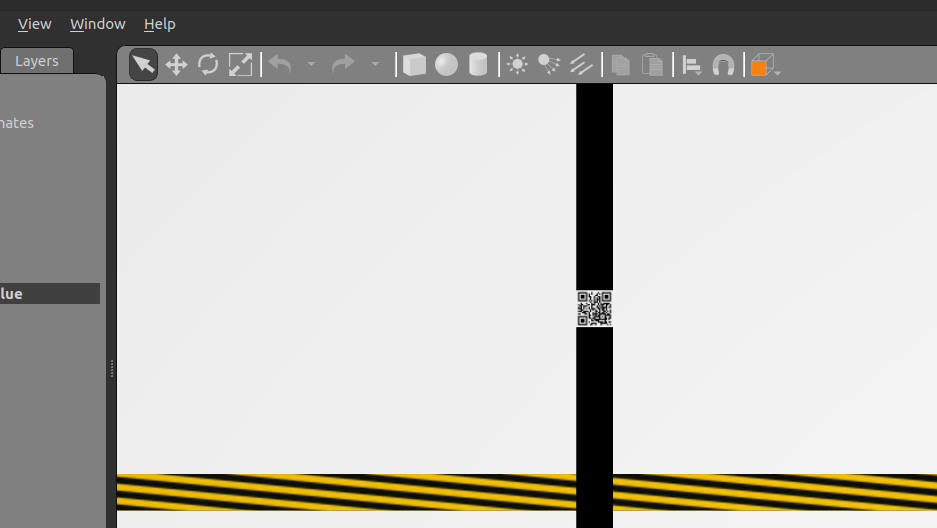
\includegraphics[width=\textwidth]{fig/qr_code_tag.png}
    \caption{Example of Qr Code tag before a loading point}
    \label{Qr Code tags} % Unique label for referencing
    \end{figure}

    the \texttt{<friction>} tag parameters of the white floor, displayed in \cref{White wooden floor}, 
were specifically chosen to replicate the conditions of wood flooring. 
The static friction coefficient was set to 0.4, representing the 
resistance to the start of sliding motion. The dynamic friction coefficient was set 
to 0.35, modeling the friction while the robot is already sliding. These values were 
carefully selected to ensure that the robot's interactions with the floor behave as 
expected in real-world conditions.

The \texttt{<static>} tag ensures that the floor model is fixed and does not move 
during the simulation. The \texttt{<pose>} tag is used to position the floor in the 
environment, placing it just slightly above the ground to avoid collision with the 
ground plane. The \texttt{<collision>} tag defines the physical properties for 
detecting interactions, including the geometry of the floor as a box shape. 
Additionally, the \texttt{<visual>} tag defines how the floor appears in the simulation, 
with the material set to a white color to represent the wooden floor's appearance. 

\newpage

\begin{minted}{xml}
    <model name='wooden_floor'>
    <static>1</static>
    <pose>0 0 0.01 0 -0 0</pose>
    <link name='floor_link'>
      <collision name='floor_collision'>
        <geometry>
          <box>
            <size>12 17 0.1</size>
          </box>
        </geometry>
        <max_contacts>10</max_contacts>
        <surface>
          <contact>
            <ode/>
          </contact>
          <bounce/>
          <friction>
            <ode/>
            <torsional>
              <ode/>
            </torsional>
            <static_friction>0.4</static_friction> <!-- Adjusted for wooden floor -->
            <dynamic_friction>0.35</dynamic_friction> <!-- Adjusted for wooden floor -->
          </friction>
        </surface>
      </collision>
      <visual name='floor_visual'>
        <geometry>
          <box>
            <size>12 17 0.1</size>
          </box>
        </geometry>
        <material>
          <ambient>1 1 1 1</ambient>
          <diffuse>1 1 1 1</diffuse>
        </material>
      </visual>
      <self_collide>0</self_collide>
      <enable_wind>0</enable_wind>
      <kinematic>0</kinematic>
    </link>
  </model>
  
\end{minted}

    \item \textbf{Obstacles and Load Platforms:} The environment includes various \textbf{obstacles} such as walls and 
    dynamic objects, designed to challenge the robot's obstacle avoidance and path planning abilities. 
    \textbf{Platforms for load dynamics} were added to simulate loading and unloading points, where the robot needs to 
    deliver or pick up objects, mimicking the tasks required during the competition.
    
    \begin{figure}[H]
        \centering
    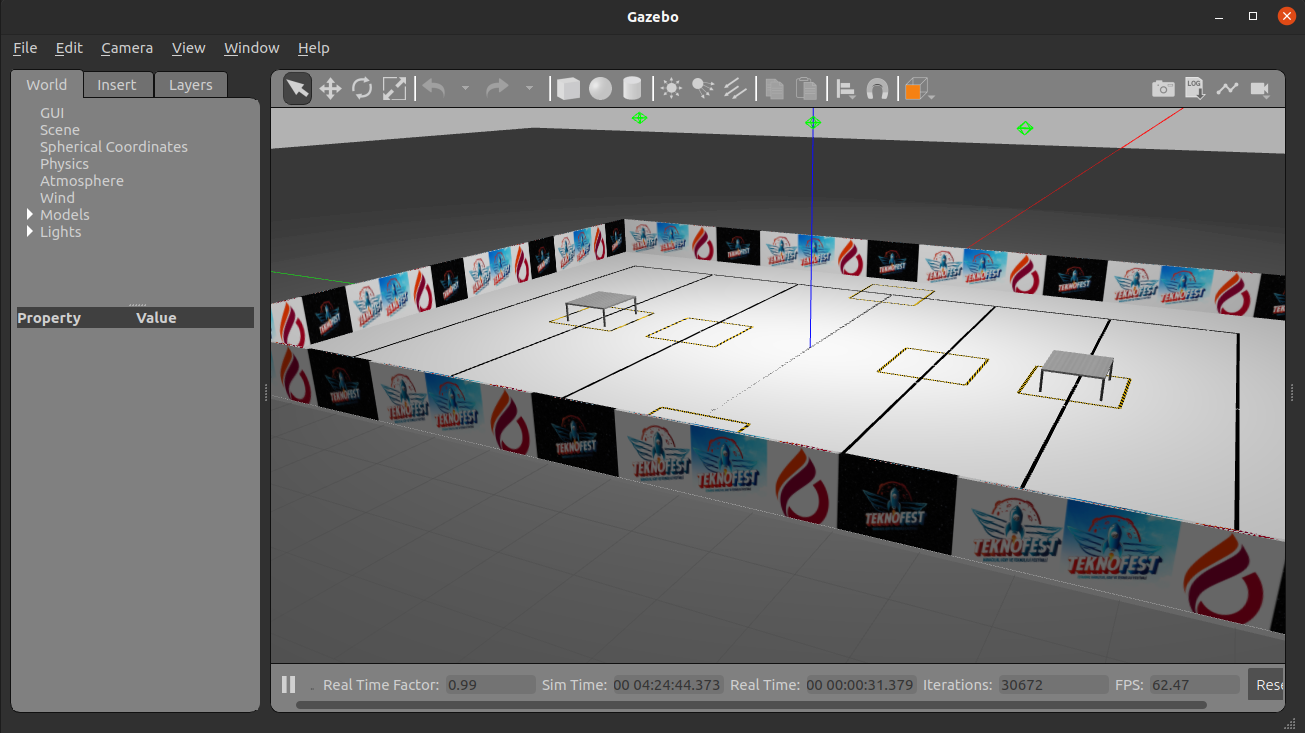
\includegraphics[width=\textwidth]{fig/walls.png}
    \caption{Competition aera bounded by ad hoardings}
    \label{Walls model} % Unique label for referencing
    \end{figure}

    \begin{figure}[H]
        \centering
    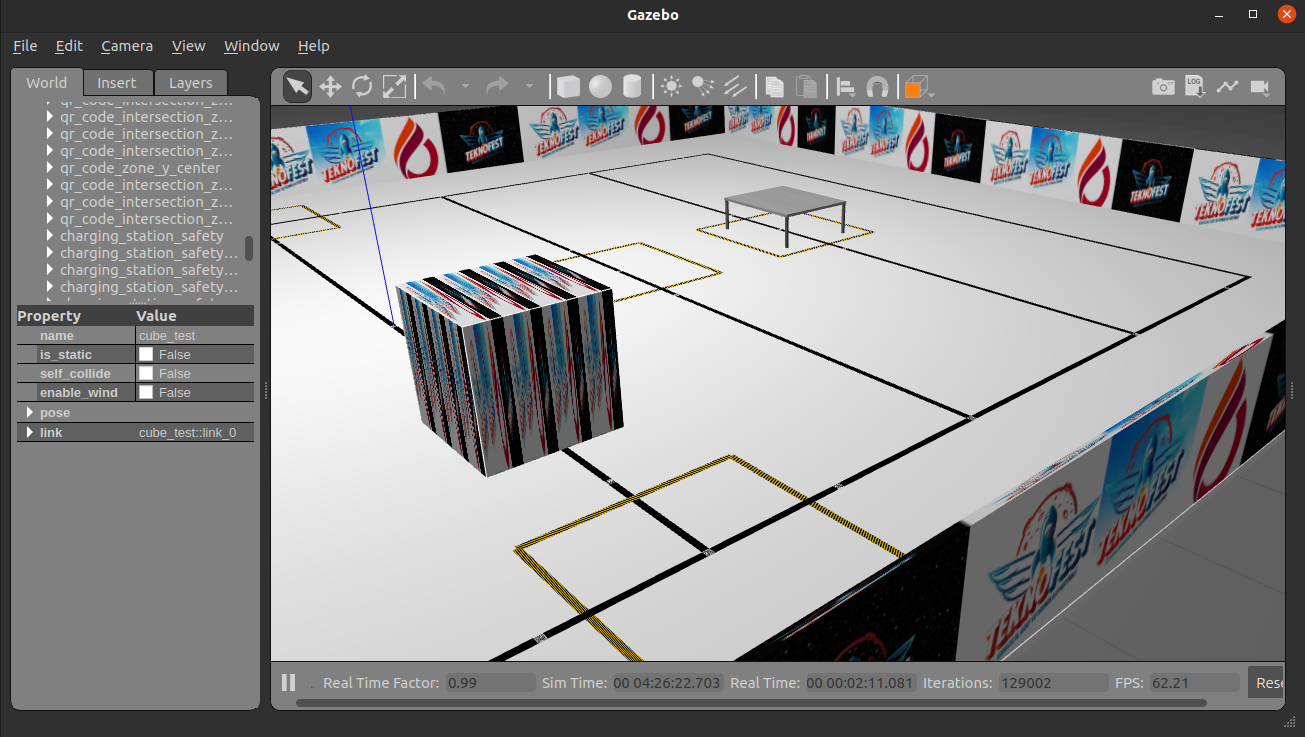
\includegraphics[width=\textwidth]{fig/load.png}
    \caption{Competition area line interrupted by permanent obstacle}
    \label{Permanent obstacle} % Unique label for referencing
    \end{figure}

    The platform model, as shown in the code snippet, is designed with a central table surface and four supporting legs. 
The structure is composed of multiple links, where each leg is defined separately, and they are all connected to the table surface through fixed joints.

The \texttt{<model>} tag defines the platform, which includes the physical properties and\\ geometric shapes of the table and legs. \\
Each link, such as \texttt{table\_surface} and \texttt{front\_left\_leg}, \texttt{front\_right\_leg}, etc., has its own inertial properties (\texttt{<inertial>}) 
and a collision geometry defined under the \texttt{<collision>} tag. 

For instance, the \texttt{<collision>} tag for the table surface has a defined friction property, with a coefficient of 1 for both static and dynamic friction, 
simulating a high-friction surface. This friction coefficient can be adjusted to simulate the specific characteristics of a material, such as wood or metal.

Each leg is represented as a cylinder, with its own collision properties and friction settings, ensuring realistic interaction with the robot 
during the simulation. The friction properties of each leg are defined in the \texttt{<surface> \texttt{<friction>}} section using \texttt{ode} settings. 
These settings also include the \texttt{<bounce>} and \texttt{<contact>} properties, which help simulate realistic physical interactions between the objects in the environment. 
Each of these legs also has a specific pose and position in the simulation.

The joints, such as \texttt{front\_left\_joint}, connect each leg to the table surface with a \texttt{fixed} type, meaning that the legs do not move relative to the table. 
The pose of each joint defines the exact position and orientation of the legs in the simulation environment.

The overall pose of the platform, including its position in the world, is defined at the end of the model, specifying the coordinates and orientation 
for the platform's placement in the simulation. 

Additionally, the platform’s visual properties are set using the \texttt{<visual>} tag, 
with a custom material representing the surface texture, such as stainless steel, applied to the table’s surface.  
To ensure accurate physical interactions, the \texttt{<inertial>} tag defines the mass and moments of inertia of the 
platform and its legs, ensuring a realistic response to forces and torques applied during the simulation.  
The \texttt{<collision>} tag specifies the geometric shape used for physics calculations, which may be simplified 
compared to the visual model to improve computational efficiency while maintaining accurate contact and 
collision responses. The platform's legs also incorporate both \texttt{<collision>} and \texttt{<inertial>} properties, 
allowing them to contribute to the overall stability of the structure while ensuring that the physics engine correctly 
simulates interactions such as impacts, weight distribution, and external forces acting on the table.  

\begin{minted}{xml}
    <model name='platform'>
      <link name='table_surface'>
        <inertial>
          <mass>13.98</mass>
          <inertia>
            <ixx>0.1</ixx>
            <ixy>0</ixy>
            <ixz>0</ixz>
            <iyy>0.1</iyy>
            <iyz>0</iyz>
            <izz>0.1</izz>
          </inertia>
          <pose>0 0 0 0 -0 0</pose>
        </inertial>
        <collision name='surface_collision'>
          <pose>0 0 0.367 0 -0 0</pose>
          <geometry>
            <box>
              <size>1.1 0.95 0.03</size>
            </box>
          </geometry>
          <surface>
            <friction>
              <ode>
                <mu>1</mu>
                <mu2>1</mu2>
              </ode>
              <torsional>
                <ode/>
              </torsional>
            </friction>
            <contact>
              <ode/>
            </contact>
            <bounce/>
          </surface>
          <max_contacts>10</max_contacts>
        </collision>
        ...
\end{minted}
\newpage  
\begin{minted}{xml}
        ... 
        <visual name='surface_visual'>
          <pose>0 0 0.367 0 -0 0</pose>
          <geometry>
            <box>
              <size>1.1 0.95 0.03</size>
            </box>
          </geometry>
          <material>
            <script>
              <uri>model://platform/materials/scripts</uri>
              <uri>model://platform/materials/textures</uri>
              <name>stainless_steel_texture</name>
            </script>
          </material>
        </visual>
        ...

\end{minted}

\begin{minted}{xml}
      ...
      <link name='front_left_leg'>
        <inertial>
          <mass>2.796</mass>
          <inertia>
            <ixx>0.01</ixx>
            <ixy>0</ixy>
            <ixz>0</ixz>
            <iyy>0.01</iyy>
            <iyz>0</iyz>
            <izz>0.01</izz>
          </inertia>
          <pose>0 0 0 0 -0 0</pose>
        </inertial>
        <collision name='collision'>
          <pose>0.53 0.455 0.1835 0 -0 0</pose>
          <geometry>
            <cylinder>
              <radius>0.02</radius>
              <length>0.367</length>
            </cylinder>
          </geometry>
          <surface>
            <friction>
              <ode>
                <mu>1</mu>
                <mu2>1</mu2>
              </ode>
              <torsional>
                <ode/>
              </torsional>
            </friction>
            <contact>
              <ode>
                <kp>100000</kp>
                <kd>1</kd>
              </ode>
            </contact>
            <bounce/>
          </surface>
          <max_contacts>10</max_contacts>
        </collision>
        <visual name='visual'>
          <pose>0.53 0.455 0.1835 0 -0 0</pose>
          <geometry>
            <cylinder>
              <radius>0.02</radius>
              <length>0.367</length>
            </cylinder>
          </geometry>
          <material>
            <script>
              <uri>file://media/materials/scripts/gazebo.material</uri>
              <name>Gazebo/Grey</name>
            </script>
          </material>
        </visual>
        <self_collide>0</self_collide>
        <enable_wind>0</enable_wind>
        <kinematic>0</kinematic>
      </link>
      <link name='front_right_leg'>
        <inertial>
          <mass>2.796</mass>
          <inertia>
            <ixx>0.01</ixx>
            <ixy>0</ixy>
            <ixz>0</ixz>
        ...
\end{minted}
    \newpage
    Ad hoardings and obstacles were incorporated into the environment using a simple yet effective approach. 
    A cube shape was used to create the basic geometry of these objects, with their dimensions adjusted to meet the specific requirements of the simulation. 
    Textures were applied to the cubes to give them the appearance of real-world hoardings and obstacles, 
    ensuring that they serve as realistic visual and physical barriers within the simulation. 

    These objects were assigned physical properties, such as mass and friction, 
    and collisions were defined to ensure proper interaction with the robot. 
    The hoardings and permanent obstacles were defined as static objects to 
    prevent them from moving during the simulation, ensuring they remain fixed 
    in place as intended. 

    The following lines provide an example of the visual and collision properties for the hoardings. 
    These lines demonstrate how the hoardings models were assigned the name \texttt{cube\_test} during the individual SDF design phase of the world. 
    The code defines the geometry, textures, and physical properties for the hoardings.

\begin{minted}{xml}
    ...
    model name='cube_test_clone_clone'>
      <link name='link_0'>
        <inertial>
          <mass>1</mass>
          <inertia>
            <ixx>0.166667</ixx>
            <ixy>0</ixy>
            <ixz>0</ixz>
            <iyy>0.166667</iyy>
            <iyz>0</iyz>
            <izz>0.166667</izz>
          </inertia>
          <pose>0 0 0 0 -0 0</pose>
        </inertial>
        <pose>-0 -0 0 0 -0 0</pose>
        <visual name='visual'>
          <pose>0 0 0 0 -0 0</pose>
          <geometry>
            <box>
              <size>0.05 16.9 1</size>
            </box>
          </geometry>
          <material>
            <lighting>1</lighting>
            <script>
              <uri>model://cube_test/materials/scripts</uri>
              <uri>model://cube_test/materials/textures</uri>
              <name>teknofest_logo</name>
            </script>
            <shader type='pixel'/>
          </material>
          <transparency>0</transparency>
          <cast_shadows>1</cast_shadows>
        </visual>
        <collision name='collision'>
          <laser_retro>0</laser_retro>
          <max_contacts>10</max_contacts>
          <pose>0 0 0 0 -0 0</pose>
          <geometry>
            <box>
              <size>0.05 16.9 1</size>
            </box>
          </geometry>
          <surface>
            <friction>
              <ode>
                <mu>1</mu>
                <mu2>1</mu2>
                <fdir1>0 0 0</fdir1>
                <slip1>0</slip1>
                <slip2>0</slip2>
              </ode>
              <torsional>
                <coefficient>1</coefficient>
                <patch_radius>0</patch_radius>
                <surface_radius>0</surface_radius>
                <use_patch_radius>1</use_patch_radius>
                <ode>
                  <slip>0</slip>
                </ode>
              </torsional>
            </friction>
            <bounce>
              <restitution_coefficient>0</restitution_coefficient>
              <threshold>1e+06</threshold>
            </bounce>
            <contact>
              <collide_without_contact>0</collide_without_contact>
              <collide_without_contact_bitmask>1</collide_without_contact_bitmask>
              <collide_bitmask>1</collide_bitmask>
              <ode>
                <soft_cfm>0</soft_cfm>
                <soft_erp>0.2</soft_erp>
                <kp>1e+13</kp>
                <kd>1</kd>
                <max_vel>0.01</max_vel>
                <min_depth>0</min_depth>
              </ode>
              <bullet>
                <split_impulse>1</split_impulse>
                <split_impulse_penetration_threshold>-0.01</split_impulse_penetration_threshold>
                <soft_cfm>0</soft_cfm>
                <soft_erp>0.2</soft_erp>
                <kp>1e+13</kp>
                <kd>1</kd>
              </bullet>
            </contact>
          </surface>
        </collision>
        <self_collide>0</self_collide>
        <enable_wind>0</enable_wind>
        <kinematic>0</kinematic>
      </link>
      <static>1</static>
      <allow_auto_disable>1</allow_auto_disable>
      <pose>-6.06431 0.045196 0.46 0 -0 0</pose>
      <enable_wind>0</enable_wind>
     </model>
     ...
\end{minted}
The design of the QR codes followed a similar approach to most other models in the 
world. Each QR code was represented by a textured cube, with textures made to 
resemble the unique images that contain the right location information.
\newpage
    \begin{minted}{xml}
      <?xml version='1.0'?>
      <sdf version='1.7'>
        <model name='qr_code'>
          <link name='link_0'>
            <pose>0 0 0 0 0 0</pose>
            <visual name='visual'>
              <pose>0 0 0 0 0 0</pose>
              <geometry>
                <box>
                  <size>0.05 0.05 0.001</size>  <!-- Increase size of the box -->
                </box>
              </geometry>
              <material>
                <lighting>1</lighting>
                <script>
                  <uri>model://qr_code/materials/scripts</uri>
                  <uri>model://qr_code/materials/textures</uri>
                  <name>qr_code_content</name>
                </script>
                <shader type='pixel'/>
              </material>
              <transparency>0</transparency> 
              <cast_shadows>1</cast_shadows>
            </visual>
          </link>
          <static>1</static>
          <allow_auto_disable>1</allow_auto_disable>
        </model>
      </sdf>
    
    \end{minted}

The above SDF code represents the individual model of the QR code. It contains 
only visual information and does not define any physical properties, as the QR 
code is used for location identification within the simulation. The model is defined 
as static to prevent movement and includes a texture that simulates the unique QR 
code image.

To simplify the referencing of points on the map in \cref{Teknofest competition real map layout}, the area was divided into several
well-defined zones. This subdivision facilitates the robot's movement management by
allowing specific tasks to be assigned to each zone. All tags were then 
assigned unique values based on their relative locations to critical
points such as loading/unloading stations, intersections, and key passage points.
These QR codes serve as essential reference markers, enabling the robot’s localization
system to determine its exact position and adjust its trajectory accordingly.

\begin{itemize}
\item \textbf{Station 1:} Located between corners 1 and 4, this zone represents station 1.
\item \textbf{Station 2:} Located between corners 2 and 3, this zone corresponds to station 2.
\item \textbf{Zone A:} Contains the loading/unloading point A.
\item \textbf{Zone B:} Contains the loading/unloading point B.
\item \textbf{Zone C:} Contains the loading/unloading point C.
\item \textbf{Zone D:} Contains the loading/unloading point D.
\end{itemize}

The QR code's content is specified using a \texttt{material} element in the SDF model. 
The \texttt{qr\_code\_contents.material} file defines the texture that represents the unique 
image of the QR code. The \texttt{material} file is referenced within the visual element of the 
QR code model using a \texttt{<script>} tag, which links to the texture folder containing 
the QR code images.

By separating the texture definition into the \texttt{qr\_code\_contents.material} 
file, it allows for easy updates and maintenance of the QR codes used in the simulation 
without needing to modify the main model files. 

    \begin{minted}{cpp}
      ...
      {
        texture_unit
        {
          texture intersection_zone_c_station_1.png
        }
      }
    }
  }
  
  material intersection_zone_c_station_2
  {
    technique
    {
      pass
      {
        texture_unit
        {
          texture intersection_zone_c_station_2.png
        }
      }
    }
  }
  
  material intersection_zone_d_station_1
  {
    technique
    {
      pass
      {
        texture_unit
        {
          texture intersection_zone_d_station_1.png
        }
      }
    }
  }
  
  material intersection_zone_d_station_2
  {
    technique
    {
      pass
      {
        texture_unit
        {
          texture intersection_zone_d_station_2.png
        }
      }
    }
  }
  
  material intersection_zone_x_station_1
  {
    technique
    {
      pass
      {
        texture_unit
        {
          texture intersection_zone_x_station_1.png
        }
      }
    }
  }
  
  material intersection_zone_x_station_2
  {
    technique
    {
      pass
      {
        texture_unit
        {
          texture intersection_zone_x_station_2.png
        }
      }
    }
  }
  
  material intersection_zone_y_station_1
  {
    technique
    {
      pass
      {
        texture_unit
        {
          texture intersection_zone_y_station_1.png
        }
      }
    }
  }
  
  material intersection_zone_y_station_2
  {
    technique
    {
      pass
      {
        texture_unit
        {
          texture intersection_zone_y_station_2.png
        }
      }
    }
  }
  ...
\end{minted}


    \begin{figure}[H]
      \centering
  
\includegraphics[width=0.4\textwidth]{fig/intersection_zone_c_station_2.png}
  \caption{Qr code tag placed at the intersection of line of the zone C and the station 2 }
  \label{Qr code tag example} % Unique label for referencing
  \end{figure}


    \item \textbf{Random Clutter Generation:} Procedural generation methods were used to add \textbf{random clutter}, 
    simulating items or obstacles that may appear unpredictably, requiring the robot to adapt to ever-changing environments. 
    
    \item \textbf{Real-World Simulation Features:} External environmental factors such as wind were not simulated,  
    as the competition setting assumes an indoor environment.  
    Basic ambient and directional lighting were configured to ensure  
    consistent visibility for sensor-based perception tasks.  
    
    Poor lighting similar to conditions in \cref{Competition area with bad lighting}~ can introduce challenges 
    such as motion blur, sensor noise, and shadow distortions,  
    making it difficult for cameras to differentiate objects from the background.  
    Additionally, extreme lighting conditions, such as glare or overexposure,  
    may lead to incorrect sensor readings, affecting navigation and localization accuracy.  
    
    \begin{figure}[H]
      \centering
  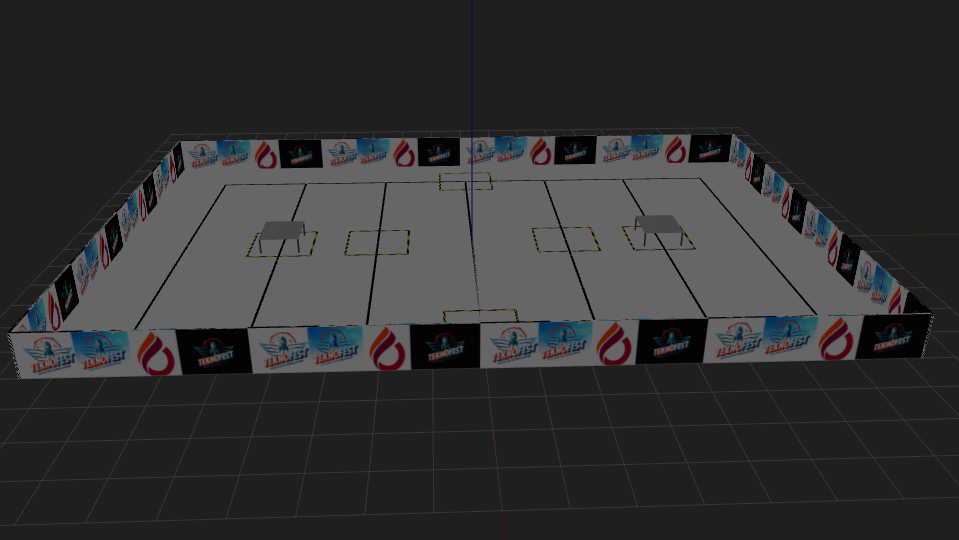
\includegraphics[width=\textwidth]{fig/competition_area_no_light.png}
  \caption{Effect of lighting conditions in simulation environment}
  \label{Competition area with bad lighting} % Unique label for referencing
  \end{figure}

    On the other hand, good lighting shown in \cref{Competition area with good lighting} improves the performance of vision-based tasks  
    such as object detection and QR code recognition.  
    A well-lit environment with uniform brightness and minimal shadows  
    ensures that cameras and sensors receive clear and consistent data,  
    reducing the chances of misinterpretation due to varying illumination levels. 
   
  \begin{figure}[H]
    \centering
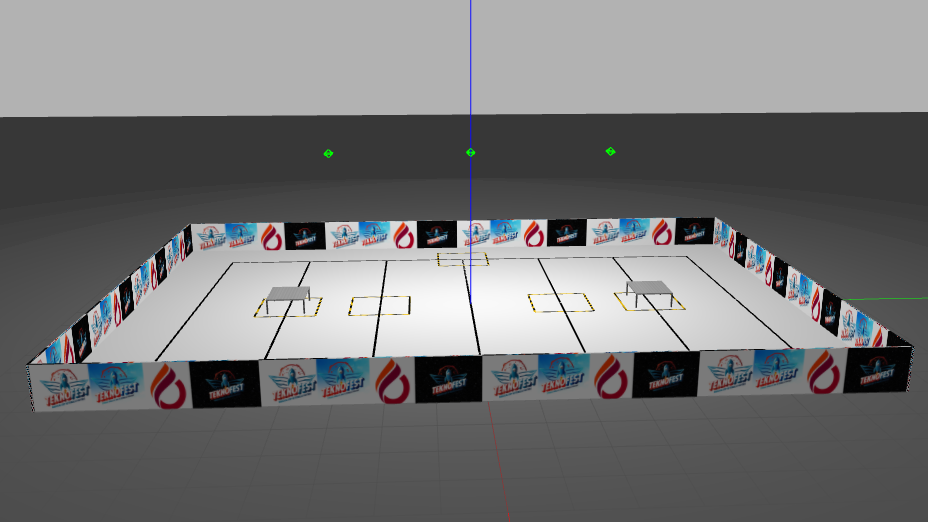
\includegraphics[width=\textwidth]{fig/competition_area_light.png}
\caption{Effect of lighting conditions in simulation environment}
\label{Competition area with good lighting} % Unique label for referencing
\end{figure}
   \end{itemize}

\subsubsection{Physics Configuration}  
I should maybe say more about this 
\subsubsection{Realism Enhancements}  
Is it necessary ? 

\subsection{Control and sensor Integration} 

You should be able to do something about this 

\section{Validation of the simulation}

\section{Challenges and Solutions} 
  
\end{document}